\chapter{Diseño Electromecánico} \label{chap:Electronica}
\chapterimage{figuras/ImagenesPortada/PortadaElectronica.jpg}
\hrule
\vspace{3mm}

Aunque se han anticipado tanto textualmente como a través de imágenes algunas características de los componentes electrónicos utilizados aún no se han descrito en detalle. Este capítulo se mete de lleno en los aspectos electromecánicos del brazo robótico, haciendo una descripción de los componentes empleados, algunas pautas para su correcto uso así como su integración dentro de la estructura descrita en el capítulo \ref{chap:Mecanica}.

\section{Actuadores} \label{sec:Electronica:Actuadores}
\label{sec:Electronica:Actuadores:G15}

    La imposición de utilizar unos motores de par reducido puede interpretarse como una desventaja, pero en este caso al quedar descartados los motores de corriente contínua y motores paso a paso convencionales queda la alternativa de uso de \glosarioPlural{smartservo} con todas las ventajas que ofrecen.
    \\

    Los \glosarioPlural{smartservo} elegidos para el proyecto son, concretamente, los G15 Cube de la marca Cytron. Estos servos vienen acompañados de una gran variedad de funcionalidades que facilitarán el control y manejo del brazo robótico. Estos servos, como la mayoría de \glosarioPlural{smartservo}, tienen implementado un sistema de comunicación bidireccional con la placa controladora a través de un tipo de comunicación conocida como \ingles{Half Serial Duplex Communication}. Como se cuenta en \cite{embeddedSystems}, este tipo de comunicación utiliza un solo cable que podrá operar en una u otra dirección cada vez. Puede darse la situación en que varios componentes intenten comunicar al mismo tiempo en ambas direcciones pudiendo ocasionar graves problemas en la electrónica de los mismos. El uso de este tipo de servos implica el uso de electrónica adicional, no solo a modo de etapa de potencia, si no para la gestión de la comunicación entre los mismos y el microcontrolador.
    \\

    Utilizar un protocolo de comunicación más complejo permite conectar varios servos a un mismo puerto de comunicación, conectando cada servo al anterior, también conocido como conexión \ingles{daisy chain}. En la figura \ref{fig:Electronica:bus-servos} se puede ver representada este tipo de cadena y donde se puede ver el aspecto del modelo de servos seleccionado.
    \\

    \begin{figure}[H]
    	\centering
    	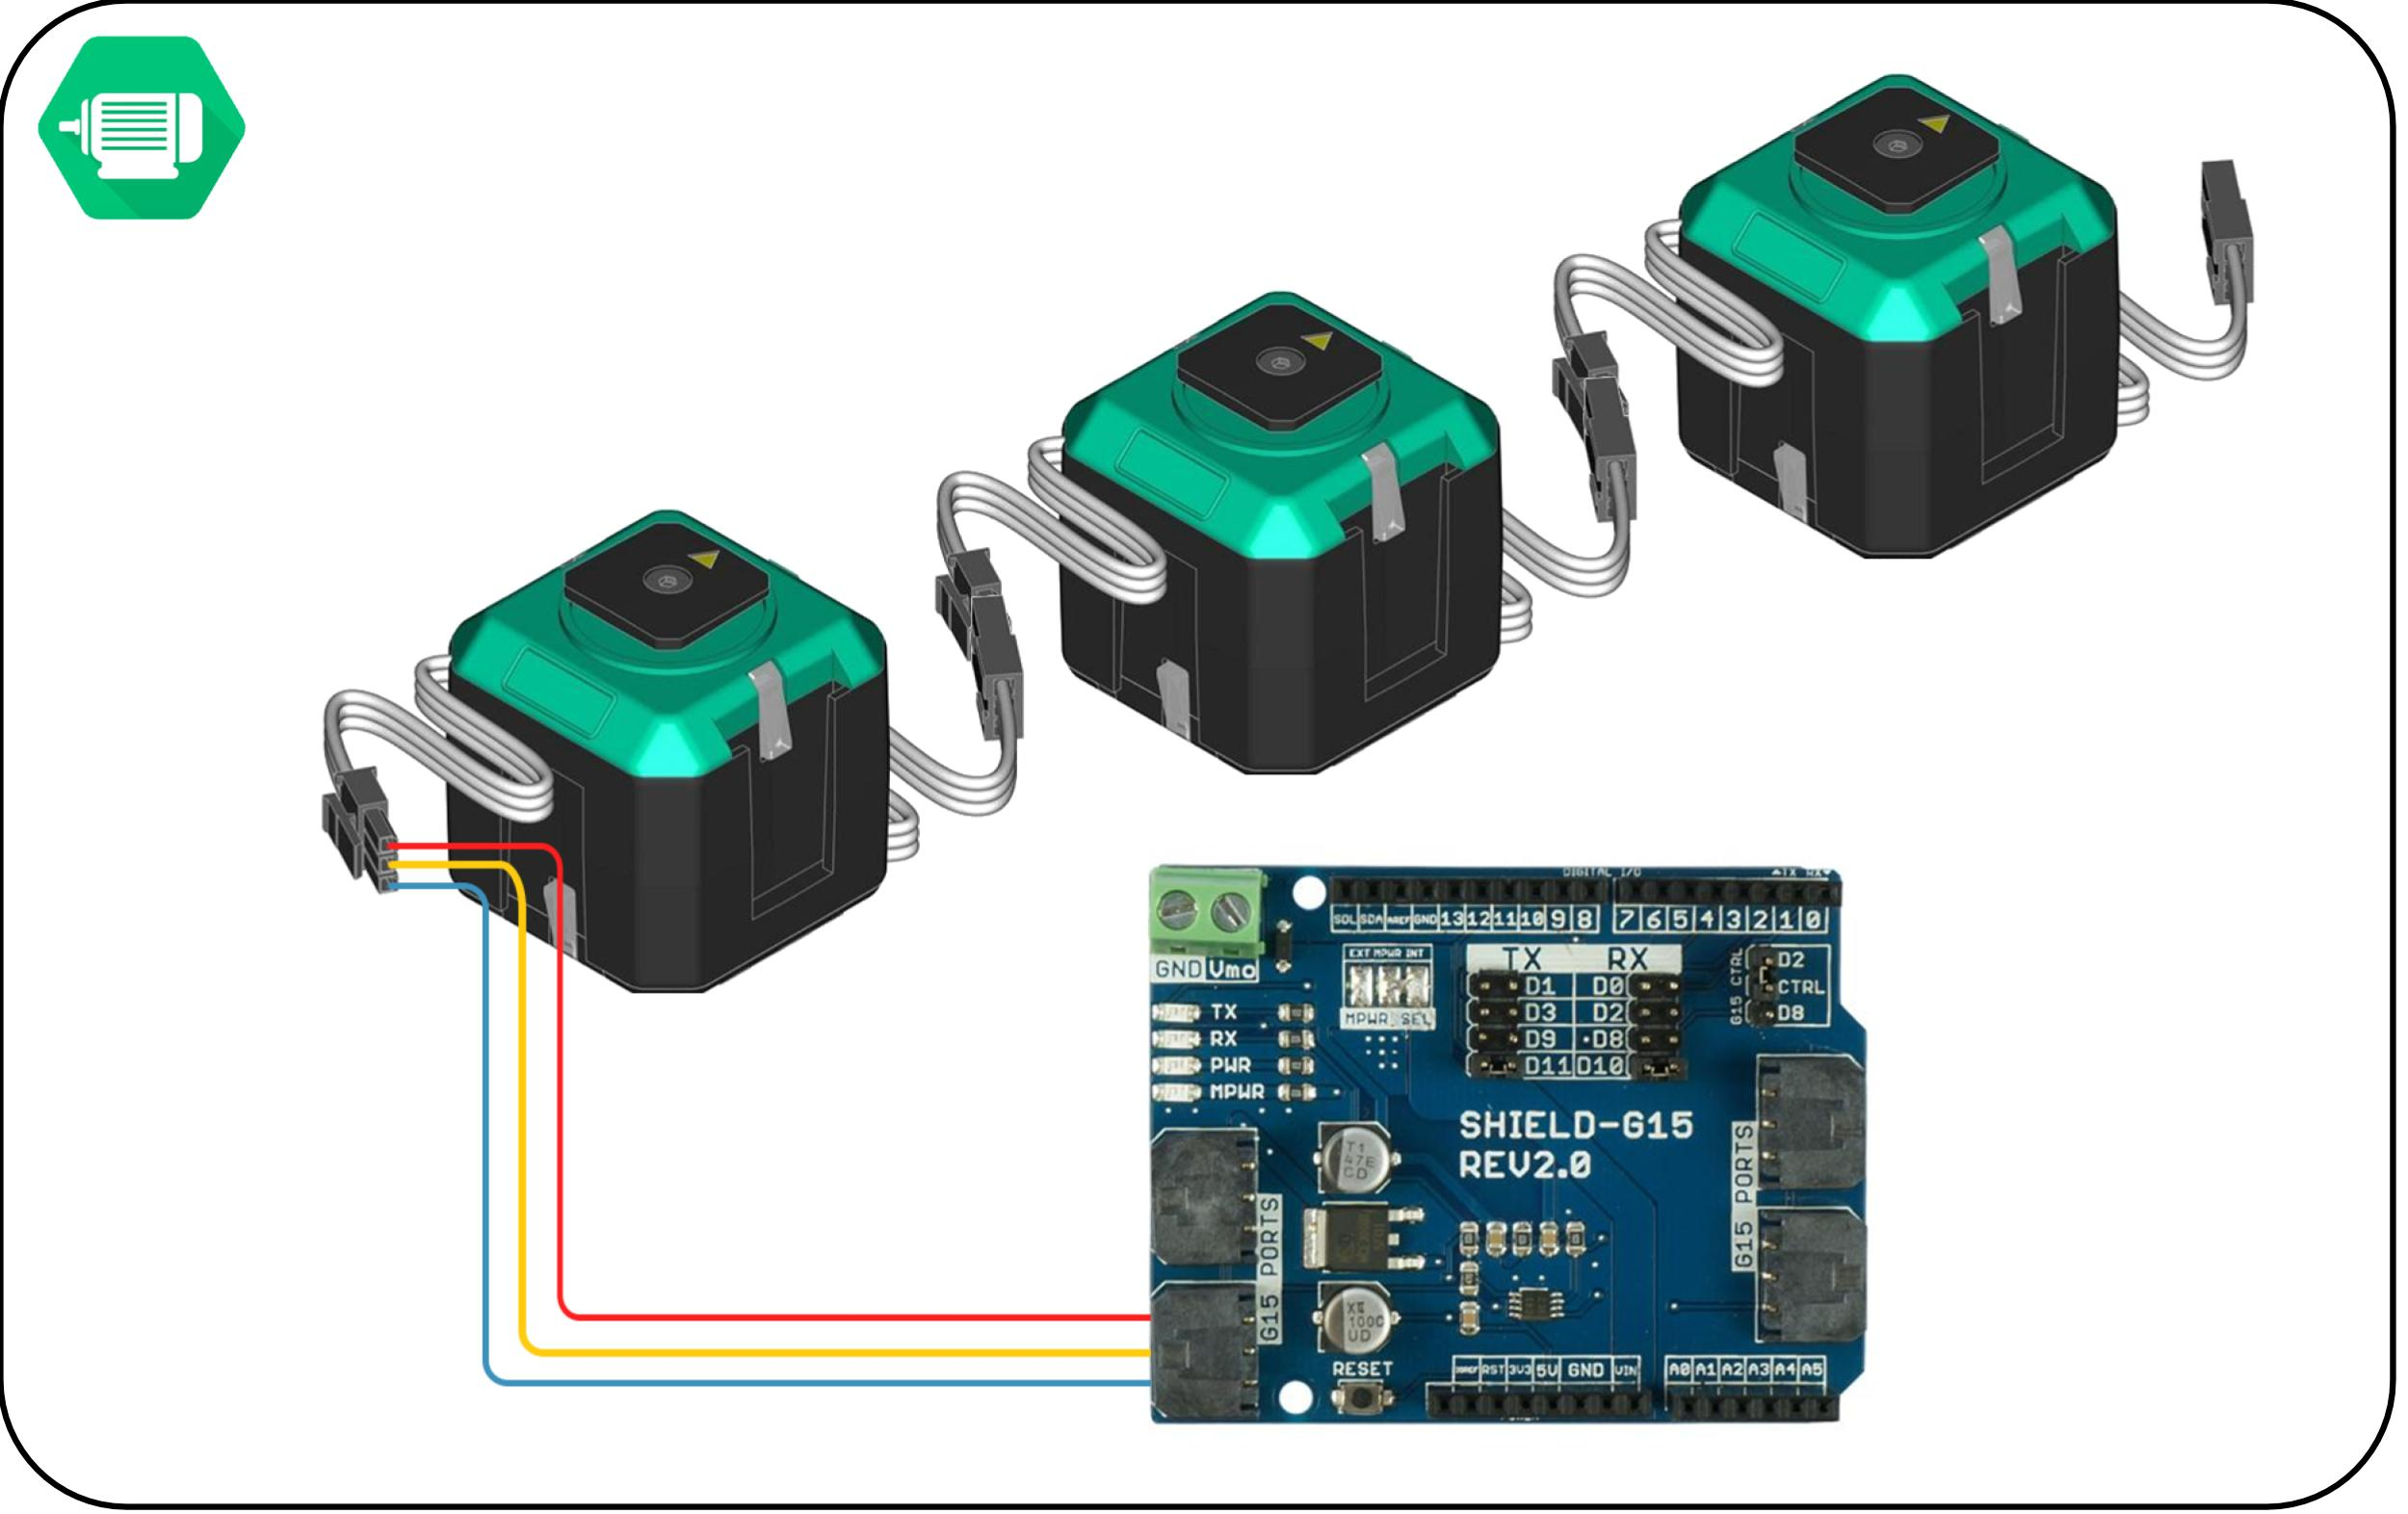
\includegraphics[width=0.8\textwidth]{figuras/Imagenes_Electronica/G15_bus_conection.jpg}
    	\caption{Esquema de la conexión de los servos formando un bus serie de servos y la placa \ingles{Shield}}
    	\label{fig:Electronica:bus-servos}
    	\immagesource{Montaje del Autor a partir de imágenes del fabricante}
    \end{figure}

    Para hacer efectiva la comunicación los servos G15 Cube cuentan con dos puertos de tres cambles cada uno. Cada uno cuenta con un conector de aspecto y forma diferente que fuerzan las conexiones en un mismo sentido siempre de forma inequívoca. Estos tres cables, como se puede ver en la imagen \ref{fig:Electronica:conectores-servos}, son utilizados para alimentación, referencia a tierra y canal de información.
    \\

    \begin{figure}[H]
    	\centering
    	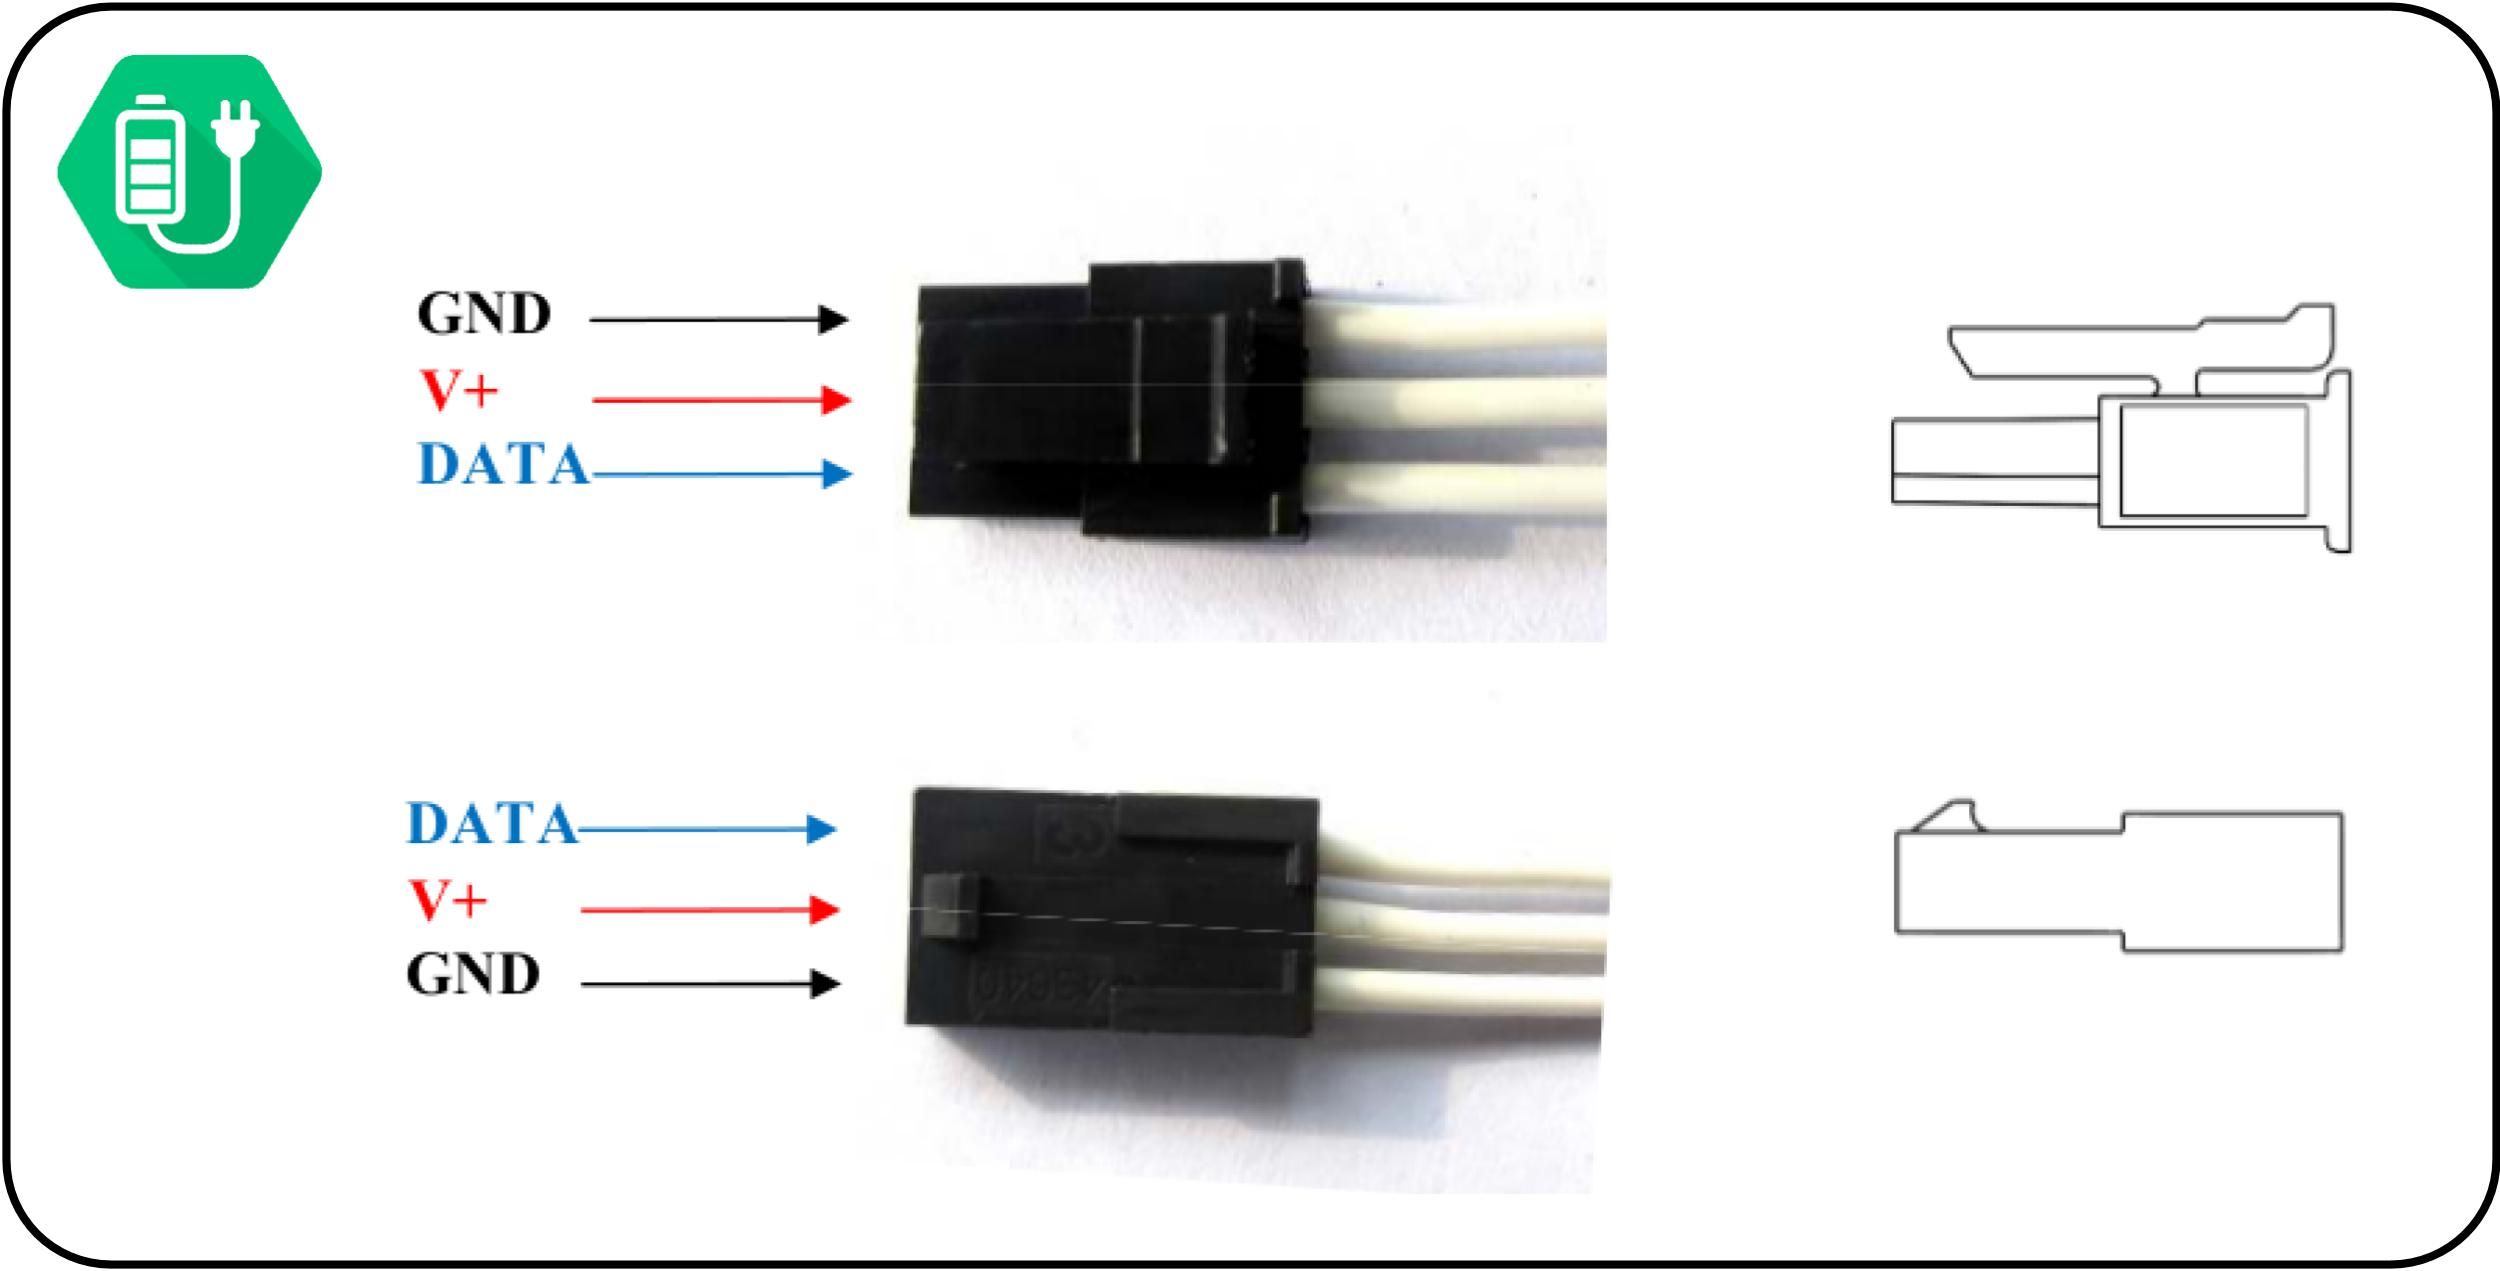
\includegraphics[width=0.7\textwidth]{figuras/Imagenes_Electronica/conectores_servos.jpg}
    	\caption{Conectores de los G15 Cube y uso de cada uno de los cables}
    	\label{fig:Electronica:conectores-servos}
    	\immagesource{Captura obtenida de \cite{CytronTechnologies2012}}
    \end{figure}

    Entre las ventajas de utilizar \glosarioPlural{smartservo} es que se cuenta con información re\-levante que se podrá \textit{preguntar} al servo cuando sea necesaria. Estos servos tienen diferentes modos de funcionamiento, aunque se utilizará principalmente el modo de \textbf{giro continuo}. Para este caso los servos ofrecen un control en par de manera que se podrán enviar comandos del par que deberá ejercer. Como información relevante a consultar ofrece datos de posición del servo, par realizado y sentido del mismo, temperatura, voltaje de alimentación, velocidad y sentido de movimiento, entre otros.
    \\

    Cabe destacar algunas características importantes de los mismos, que se encuentran resumidas en la tabla \ref{tab:g15_catact}. Concretamente es de destacar los $12kg \cdot cm$ de par efectivo; un par relativamente bajo que se aprovechará como medida extra de protección a usuarios del brazo robótico tal y como se ha anticipado en capítulos anteriores.

    \begin{table}[H]
    	\caption{Características relevantes de los Servos G15 de Cytron.}
    	\immagesource{Tabla traducida y resumida de \cite{CytronTechnologies2012}}
    	\label{tab:g15_catact}
   		\begin{minipage}{0.42\textwidth}
   		\begin{center}
   		\begin{tabular}{ |c|c|c|c| }
			\hline
			\multicolumn{4}{|c|}{\textbf{Características eléctricas}} \\
			\hline
			\textbf{Parámetro} & \textbf{Valor Mínimo} & \textbf{Valor Típico} & \textbf{Valor Máximo} \\
			\hline
			Voltaje & $6.5V$ & $12V$ & $17.8V$ \\
			\hline
			Consumo de corriente ($12V$) & & & $1.5A$ \\
			\hline
			Temperatura de funcionamiento & $0^oC$ & & $80^oC$ \\
			\hline
			\multicolumn{4}{c}{\textbf{}} \\
			\hline
			\multicolumn{4}{|c|}{\textbf{Especificaciones técnicas}} \\
			\hline
			\multicolumn{2}{|c|}{Peso} & \multicolumn{2}{|c|}{$63g$}\\
			\hline
			\multicolumn{2}{|c|}{Par capaz de realizar (a $12V$)} & \multicolumn{2}{|c|}{$12kg \cdot cm$}\\
			\hline
			\multicolumn{2}{|c|}{Par capaz de soportar} & \multicolumn{2}{|c|}{$15kg \cdot cm$} \\
			\hline
			\multicolumn{2}{|c|}{Margen angular de operación } & \multicolumn{2}{|c|}{$360^o$ en giro continuo}\\
			\hline
			\multicolumn{2}{|c|}{Máxima velocidad (en vacío a $12V$)} & \multicolumn{2}{|c|}{$63 RPM$ }\\
			\hline
			\multicolumn{2}{|c|}{Comunicación} & \multicolumn{2}{|c|}{ \begin{minipage}{1.0\textwidth}\vspace{0.1cm}
			Half duplex asynchronous serial \\ communication ($7812.5bps-500kbps $)\end{minipage} }\\
    		\hline
    	\end{tabular}
   		\end{center}
   		\end{minipage}
    \end{table}

    Como curiosidad extra, este modelo de servos presenta la particularidad de estar diseñados de forma modular; así podrán ser apilados de diferentes maneras entre ellos.

\section{Interfaz servos-microcontrolador} \label{sec:Electronica:Potencia}

	Pasada la descripción de los actuadores, los G15 Cube Servo, se hace patente la necesidad de una etapa intermedia entre la placa controladora y los servos que gestione la comunicación entre ambos de forma segura y que desacople la alimentación del controlador de la alimentación de los servos, que requieren un voltaje de 12V (ver \ref{tab:g15_catact}).
	\\

	Es la propia marca que fabrica los servos, Cytron Technologies, la que suministra una placa auxiliar o \ingles{shield} con este propósito. Concretamente se utilizará la segunda generación de dicha placa, vista en la figura \ref{fig:Electronica:bus-servos} de la sección anterior.
	\\

	Para la alimentación de los servos se ofrecen dos posibles entradas remarcadas en la figura \ref{fig:Electronica:alimentacion-shield} con los colores azul y rojo. Para alternar de una a otra habrá que, mediante el uso de un soldador, modificar la conexión recuadrada en amarillo para habilitar la opción deseada deshabilitando la contraria.
	\begin{itemize}
		\item Alimentación externa (recuadrada en azul): en este caso se conecta la fuente de alimentación directamente a los conectores pasando el voltaje a los cables de alimentación de los servos.
		\item Alimentación mixta shield-controlador (recuadrada en rojo): en este caso la alimentación se comparte con la placa controladora (que deberá rectificar el voltaje de entrada a valores aceptables para la misma). Por defecto esta es la entrada que viene habilitada; se ha mantenido ya que permite la alimentación simultánea de los servos y de la placa controladora a partir de la misma fuente de alimentación (se verá en secciones posteriores la elección del controlador y otros aspectos). Esta entrada suministra los 12V necesarios para los servos a la vez que, internamente a la placa Arduino, se rectifica a 5V para la alimentación de la misma.
	\end{itemize}

	\begin{figure}[H]
		\centering
		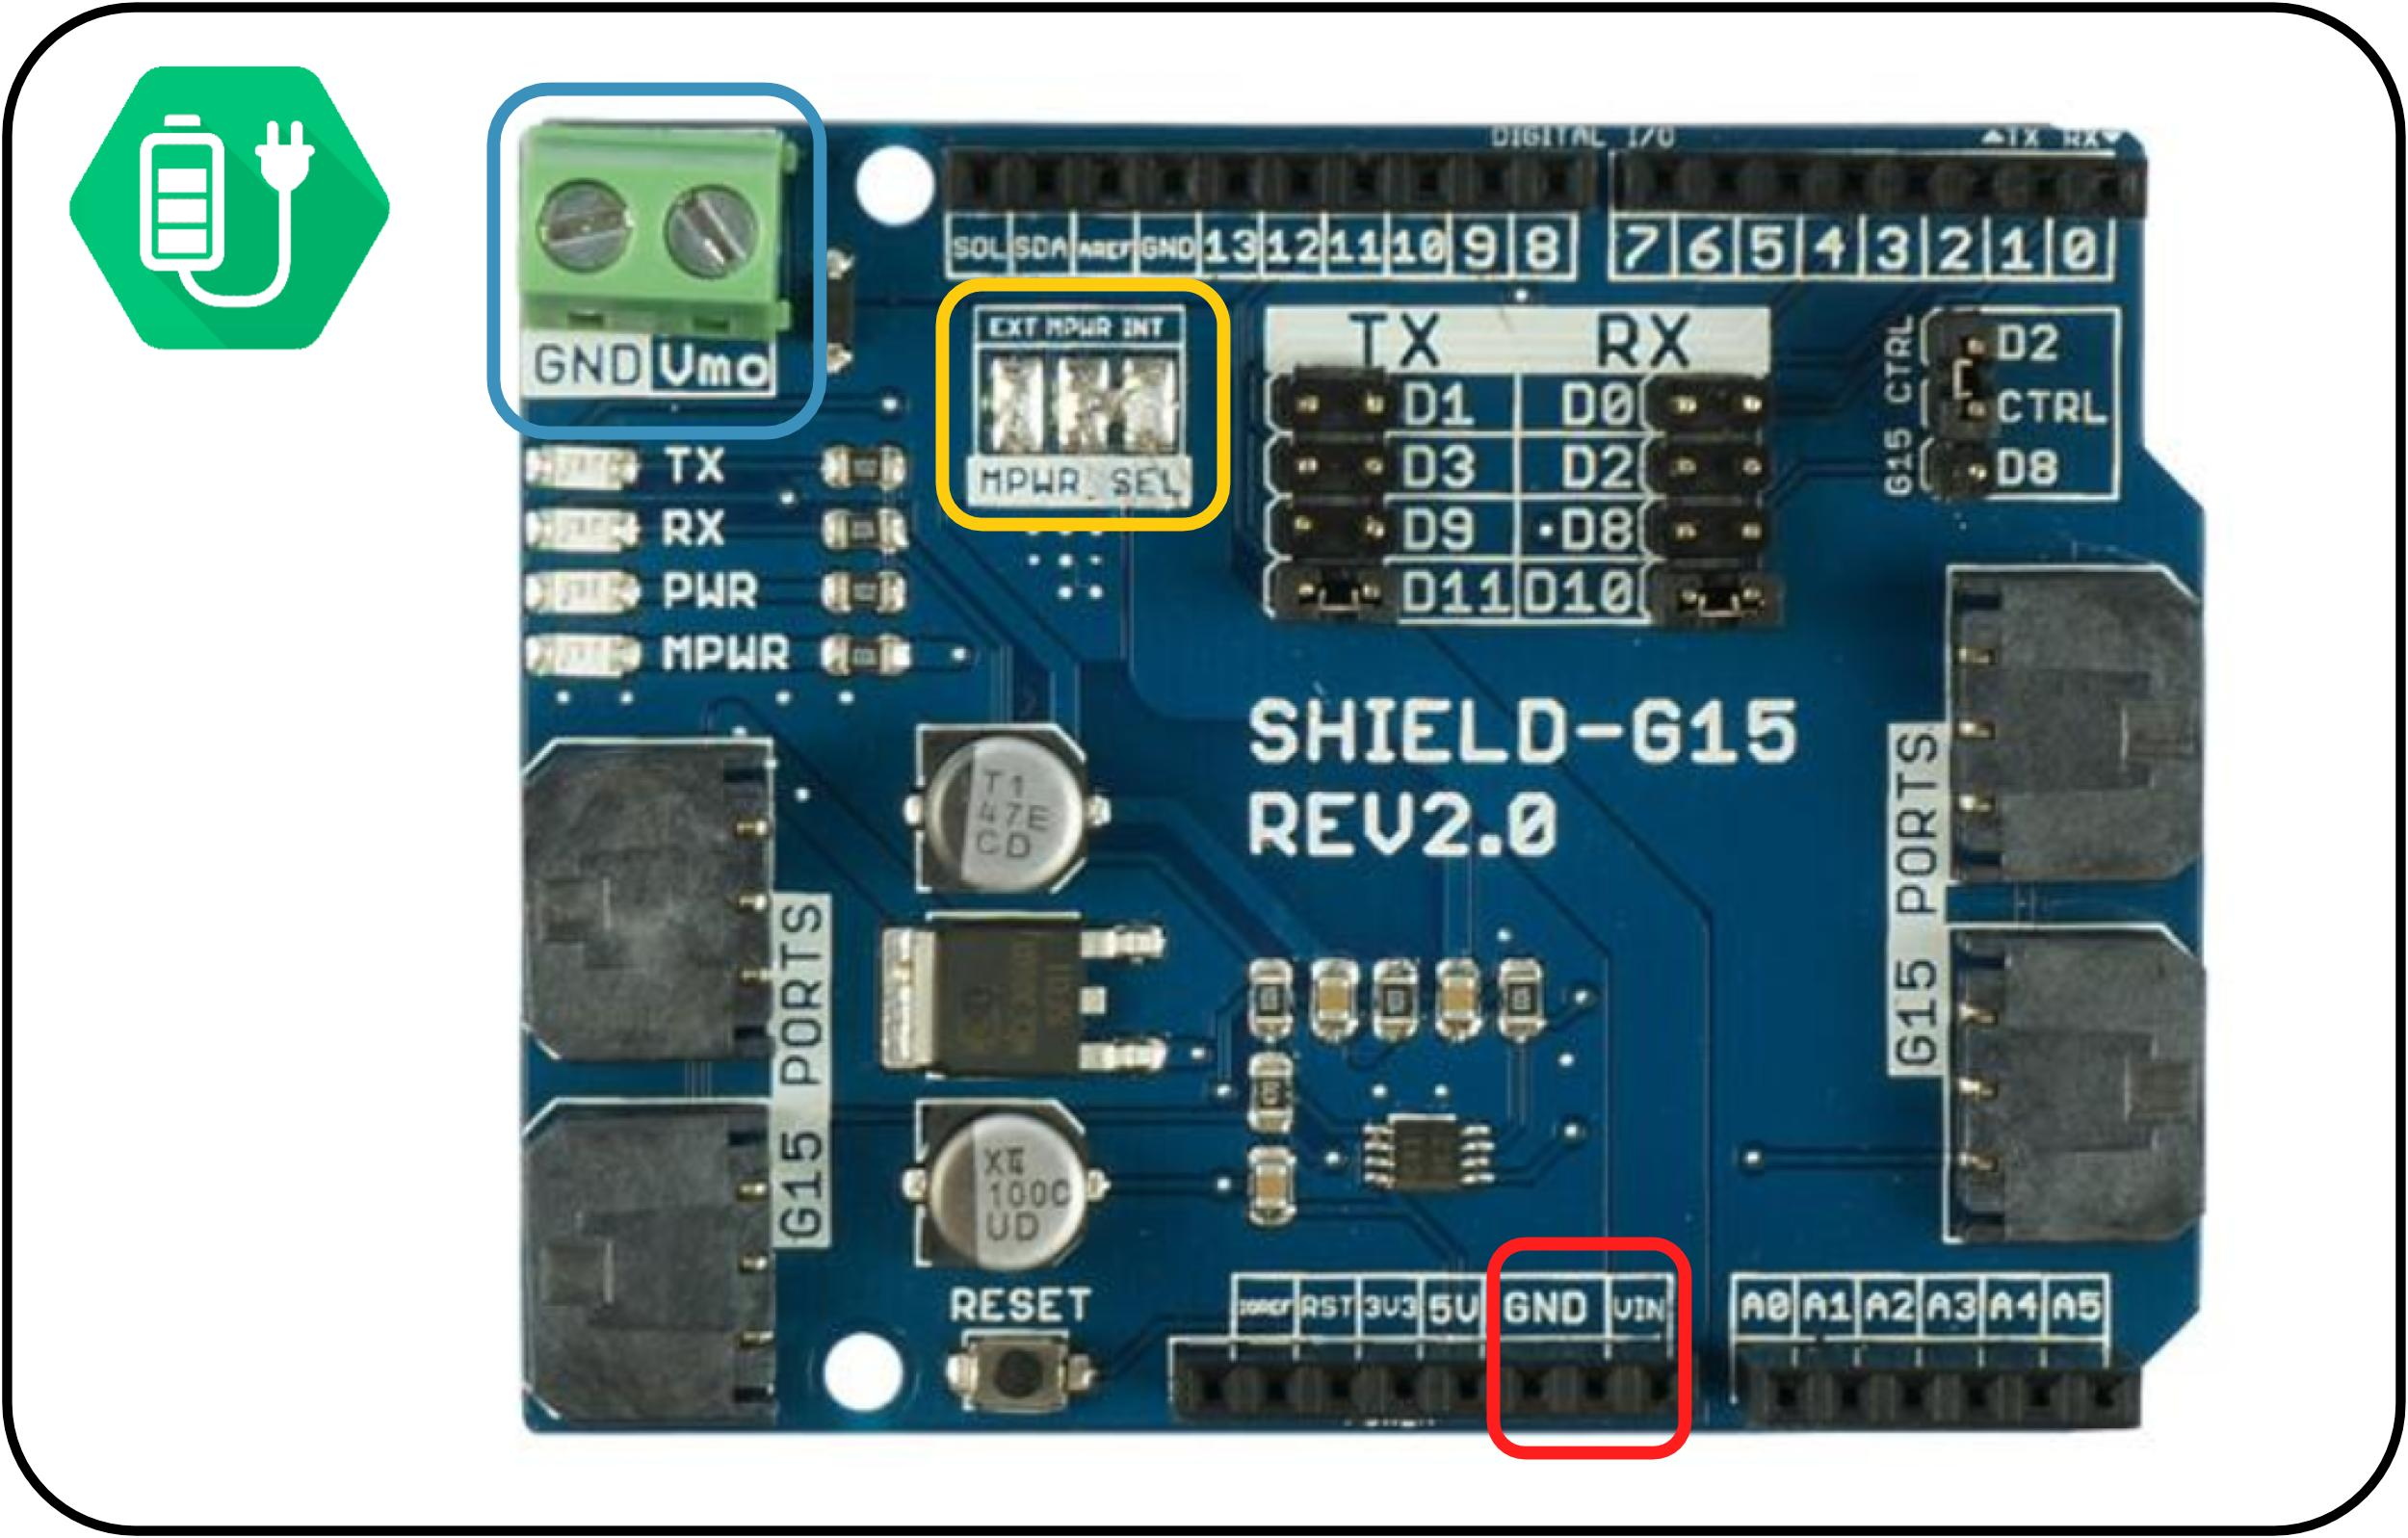
\includegraphics[width=0.7\textwidth]{figuras/Imagenes_Electronica/alimentacion-shield.jpg}
		\caption{Posibilidades para la alimentación de los servos}
		\label{fig:Electronica:alimentacion-shield}
		\immagesource{Captura obtenida de \cite{CytronTechnologies2012} y editada por el Autor del proyecto}
	\end{figure}

	En la figura \ref{fig:Electronica:alimentacion-shield} pueden distinguirse una serie de pines de conexión con las letras RX, TX y CTRL. Esta placa está pensada para funcionar a modo de interfaz entre un puerto serie común (con un cable de emisión y otro de recepción de datos) y un puerto serie de tipo \ingles{Half Duplex} como el empleado por los servos.
	\\

	Como se describe en \cite{CytronTechnologies2012} la \ingles{shield} incluye integrada un circuito integrado (concretamente el 74HC126 IC) que resuelve los problemas de comunicación inherentes a la comunicación bidireccional por un solo hilo. A través de un pin de control (CTRL en la shield) se gestiona la conexión entre el hilo del \ingles{Half Duplex} y los hilos del puerto serie alternando de uno a otro en función del estado de la señal de control (alto nivel o bajo nivel).

\section{Placa controladora} \label{sec:Electronica:Placa}

	La placa \ingles{shield} descrita en el apartado anterior está especialmente diseñada para encajar en placas tipo Arduino, concretamente el modelo Arduino Uno. En el marco de este proyecto se ha realizado una fase del desarrollo utilizando como base una placa Arduino Uno, aunque posteriormente se ha cambiado a un Arduino Mega. Más adelante se explicará la motivación de dicho cambio, pero merece volver sobre el aspecto de la alimentación de la placa descrito en el apartado anterior. Según se especifica en \cite{arduinoUno} y en \cite{arduinoMega} el voltaje de entrada recomendado abarca desde los 7 a los 12V teniendo como limitación inferior un mínimo de 6V y un máximo de 20V. En este caso se aplicarán 12V, que quedan incluidos dentro del rango recomendado por el fabricante.
	\\

	En el caso de la placa Arduino Uno la \ingles{shield} viene preparada para encajar sobre la misma. La comunicación con los servos está pensada para efectuarse de dos formas:
	\begin{itemize}
		\item A través de un puerto serie UART hardware: en el caso de la placa Arduino Uno solo dispone del puerto conectado a los pines 0 y 1, que también es el usado para la carga de software y comunicación con el ordenador, por lo que queda descartado.
		\item Emulando un puerto serie mediante software en otros pines de la placa. La \ingles{shield} trae una serie de \ingles{jumpers} \footnote{Los \ingles{jumpers} son conectores que sirven para cortocircuitar el par de pines que se desee.} que permiten cambiar entre una selección de pines para cada caso (RX, TX o CTRL).
	\end{itemize}

	Como se puede ver, utilizando una placa Arduino Uno la comunicación con los servos queda relegada a un puerto emulado por software. Esta es la razón principal por la cual se decide cambiar y utilizar una Placa Arduino Mega2560, que además presenta mayores prestaciones respecto a memoria (ver tabla \ref{tab:arduino_comparison}). Para el control del brazo robótico y el diseño y testeo del software es necesario optimizar la velocidad de comunicación entre los dispositivos al máximo. La placa Arduino Mega incluye tres puertos serie hardware adicionales que se podrán puentear a la placa \ingles{shield} para ser utilizados. Esta conexión se puede ver en la figura \ref{fig:Electronica:shield-arduino}. De esta forma se podrá aprovechar todo el potencial de la comunicación a través de un puerto serie hardware.
	\\
	
	Se utilizarán tres puertos serie de la placa: uno para comunicar con los servos, otro para la carga de software así como funcionalidades de debug para desarrollo y un tercer puerto para el control del robot a través una comunicación serial.
	\\

	Para hacerse una idea de la importancia que tiene este cambio se ha forzado la comunicación en ambos casos para obtener los máximos en los cuales sería viable trabajar. Los datos presentados en la tabla \ref{tab:comunication_serial} se han obtenido de forma experimental bajo el marco de este proyecto. Entre los mismos se puede apreciar la gran diferencia existente entre las diferentes formas de comunicación. Las velocidades se han ido duplicando (a modo de convencionalismo las velocidades de comunicación estándar para Placas Arduino suelen obtenerse de esta manera) hasta llegar al máximo que permite una comunicación satisfactoria.

	 \begin{table}[H]
	 	\caption{Comparativa entre placas Arduino Uno y Arduino Mega2560}
	 	\immagesource{Tabla con información obtenida de forma experimental }
	 	\label{tab:comunication_serial}
	 		\begin{center}
	 			\begin{tabular}{ |c|c|c| }
	 				\hline
	 				\textbf{Tipo de comunicación}& \begin{minipage}{.30\linewidth} \textbf{Velocidad máxima  en baudios}  \end{minipage}& \begin{minipage}{.30\linewidth} \textbf{Velocidad máxima en bytes/milisegundo} \end{minipage} \\
	 				\hline
	 				\begin{minipage}{.30\linewidth}\vspace{2pt} Puerto Serie \textbf{Sowtware} (AUno):  Shield-controlador \vspace{2pt} \end{minipage} & 57600 bauds & 7.2 bytes/ms \\
	 				\hline
	 				\begin{minipage}{.30\linewidth}\vspace{2pt} Puerto Serie \textbf{Hardware} (AMega):  Shield-controlador \vspace{2pt} \end{minipage} & 460800 bauds & 57.6 bytes/ms \\
	 				\hline
	 				\begin{minipage}{.30\linewidth}\vspace{2pt} Puerto Serie \textbf{Hardware} (Ambas):  controlador-ordenador \vspace{2pt} \end{minipage} & 921600 bauds & 115.2 bytes/ms \\
	 				\hline
	 			\end{tabular}
	 		\end{center}
	 \end{table}

	 En este proyecto concreto se enlazarán diferentes lazos de control a diferentes frecuencias de refresco (ver capítulo \ref{chap:Control}) que exigirán el máximo de la capacidad comunicativa entre los dispositivos. Los datos máximos obtenidos para la placa Arduino Mega son los utilizados para el funcionamiento del robot.

    \begin{figure}[H]
    	\centering
    	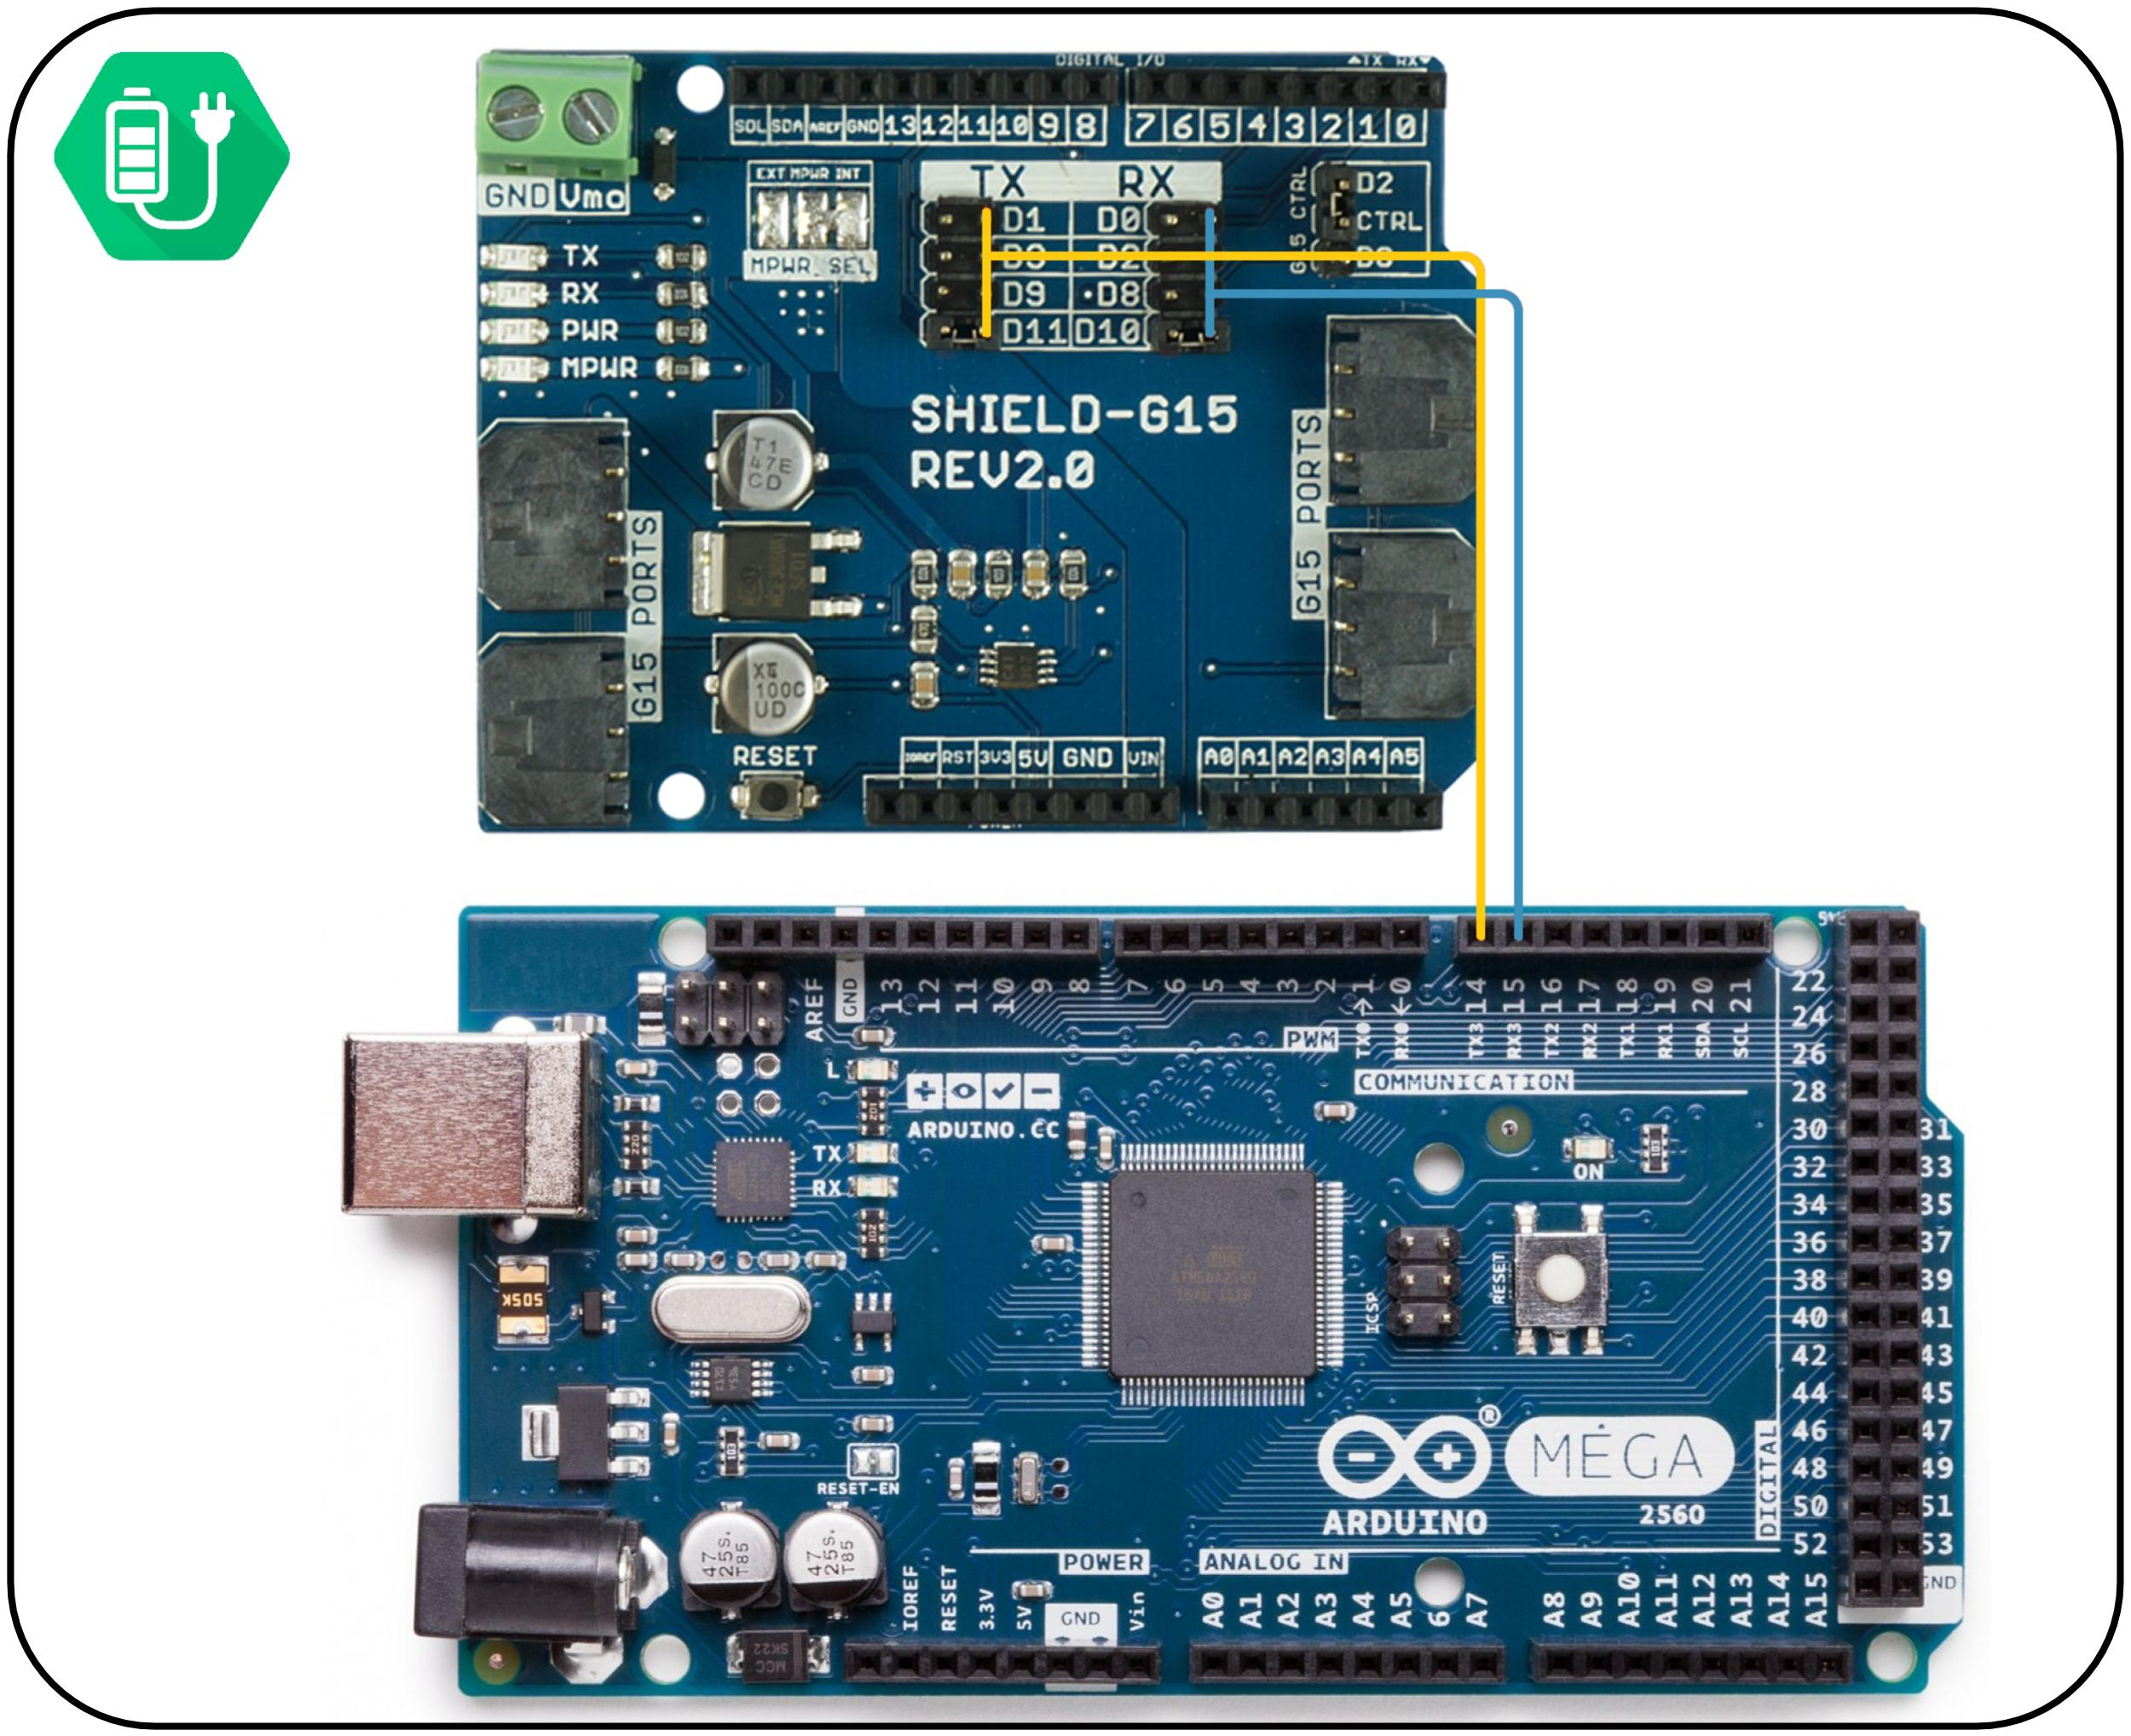
\includegraphics[width=0.75\textwidth]{figuras/Imagenes_Electronica/Shield-Arduino-Conection.jpg}
    	\caption{Esquema de la conexión entre la placa Shield y Arduino para utilizar los puertos Hardware Serie de la Arduino Mega}
    	\label{fig:Electronica:shield-arduino}
    	\immagesource{Montaje del Autor a partir de imágenes del fabricante}
    \end{figure}

    \begin{table}[H]
       	\caption{Comparativa entre placas Arduino Uno y Arduino Mega2560}
       	\immagesource{Tabla con información resumida de \cite{arduinoUno} y \cite{arduinoMega}}
       	\label{tab:arduino_comparison}
       	%\begin{minipage}{0.42\textwidth}
       		\begin{center}
       			\begin{tabular}{ |c|c|c| }
       				\hline
       				&\textbf{Arduino Uno}&\textbf{Arduino Mega2560} \\
       				\hline
       				Número de pines entrada/salida & 14 & 54 \\
       				\hline
       				Memoria flash & 32KB & 256 KB \\
       				\hline
       				SRAM & 2KB & 8KB \\
       				\hline
       				EEPROM & 1KB & 4KB \\
       				\hline
       				Velocidad de reloj & 16MHz & 16Mhz \\
       				\hline
       			\end{tabular}
       		\end{center}
       	%\end{minipage}
    \end{table}

\section{Sensores} \label{sec:Electronica:Sensores}
    A pesar de la gran cantidad de información que ofrecen los servos escogidos, por las características mecánicas descritas las medidas que proporcionan no son medidas directamente referenciadas a las articulaciones. Desde el punto de vista de control del brazo robótico el objetivo es el control del brazo completo descomponiendo el problema de control de las articulaciones. Principalmente en las articulaciones dos y tres cuya relación entre las medidas del servo y el comportamiento de la articulación es más compleja es conveniente incluir una realimentación externa, concretamente de posición.
    \\

    La realimentación se hará efectiva a través del uso de potenciómetros para ambas articulaciones. Aunque aun no se ha tratado en detalle los rangos de movimiento posibles para cada articulación, la explicación de la sección \ref{sec:Mecanica:articulacion_dostres} permite deducir que el rango de movimiento será: para el caso de la segunda articulación menor a $180^o$; para la tercera articulación menor a $90^o$. En capítulos posteriores se tratará en detalle estos aspectos del robot; es necesario anticiparse para la elección de los potenciómetros.
    \\

    El modelo de potenciómetro elegido es el modelo TW1502KA de la marca TE Connectivity (ver figura \ref{fig:Electronica:potenciometro}). Se pueden ver las características principales mostradas en \cite{potenciometroSheet} en la tabla \ref{tab:potenciometro}

    \begin{figure}[H]
    	\centering
    	
\includegraphics[width=\textwidth]{figuras/Imagenes_Electronica/potenciometro.jpg}
    	\caption{Visual del potenciómetro escogido}
    	\label{fig:Electronica:potenciometro}
    	\immagesource{Fotografía del fabricante}
    \end{figure}

    \begin{table}[H]
        \caption{Características resumidas del modelo de potenciómetro TW1502KA}
        \immagesource{Tabla con información resumida de \cite{potenciometroSheet}}
        \label{tab:potenciometro}
        %\begin{minipage}{0.42\textwidth}
            \begin{center}
                \begin{tabular}{ |c|c| }
                    \hline
                    Resistencia & $5K\Omega$  \\
                    \hline
                    Rotación (rango eléctrico) & $265^o \pm 5^o$\\
                    \hline
                    Tolerancia & 10\%  \\
                    \hline
                    Tipo de Respuesta & Lineal  \\
                    \hline
                \end{tabular}
            \end{center}
        %\end{minipage}
    \end{table}

    Se puede apreciar, que los potenciómetros escogidos cubren por completo el rango de movimiento de las articulaciones que se pretende realimentar.

\section{Fuente de alimentación} \label{sec:Electronica:fuente_alimentacion}
    Acorde con la información que se ha dado anteriormente la fuente elegida (ver figura \ref{fig:Electronica:fuente}) deberá suministrar un voltaje suficiente para la alimentación de todo el sistema. Se ha escogido el modelo S-120-12, cuyas características se pueden ver en la tabla \ref{tab:fuente}.
 
	\begin{figure}[H]
	  	\centering
	  	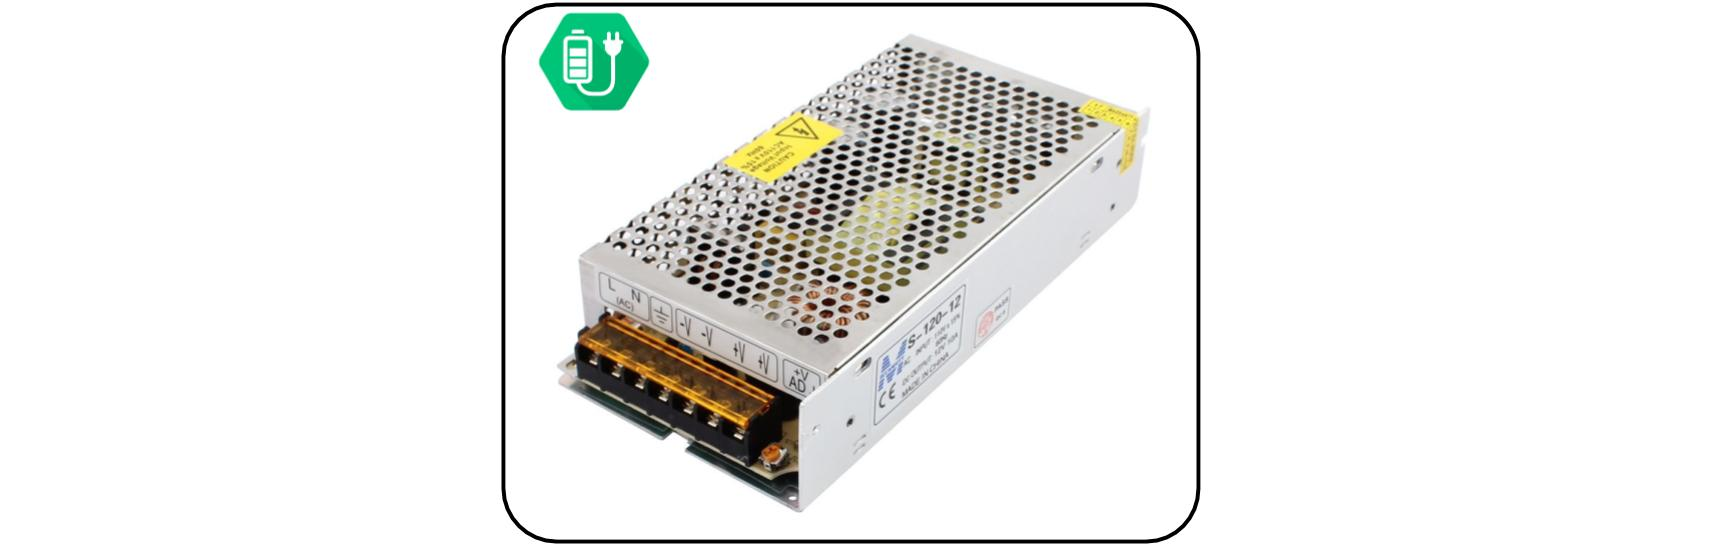
\includegraphics[width=\textwidth]{figuras/Imagenes_Electronica/fuente_alimentacion.jpg}
	  	\caption{Visual de la fuente de alimentación escogida}
	  	\label{fig:Electronica:fuente}
	  	\immagesource{Fotografía del fabricante}
	\end{figure}
	
	\begin{table}[H]
      	\caption{Características de la fuente de alimentación}
      	\immagesource{Fuente de alimentación}
      	\label{tab:fuente}
      	%\begin{minipage}{0.42\textwidth}
      	\begin{center}
      		\begin{tabular}{ |c|c| }
      			\hline
      			Voltaje de entrada & $200-240 V(AC)a$  \\
      			\hline
      			Intensidad de entrada & $1.2A$\\
      			\hline
      			Voltaje de salida & $+12V(DC)$  \\
      			\hline
      			Intensidad de salida & $10A$  \\
      			\hline
      		\end{tabular}
      	\end{center}
      	%\end{minipage}
	\end{table}
	
\section{Adaptador USB para puerto serie}
	Este componente permite adaptar los puertos serie de la placa Arduino Mega de forma que sean compatibles con una entrada USB. De esta forma se tiene acceso a los pines RX y TX a través de USB. Se utiliza para comunicar otro puerto serie extra a través de USB.
	\\
	
	En modelo de la figura \ref{fig:Electronica:ftdi} es compatible con dispositivos a 3.3V y a 5V (como es el caso de la placa utilizada).
	\begin{figure}[H]
		\centering
		
\includegraphics[width=\textwidth]{figuras/Imagenes_Electronica/adaptador_ftdi.jpg}
		\caption{Adaptador puerto serie a USB}
		\label{fig:Electronica:ftdi}
		\immagesource{Fotografía del fabricante}
	\end{figure}
\section{Integración de los componentes en la estructura mecánica} \label{sec:Electronica:Integracion}

    Una vez conocidos los componentes electromecánicos que se van a utilizar pueden ser integrados en la estructura diseñada.
    \\

    En el caso de los tres servos encargados de los grados de libertad de posición, han sido montados en una torre apoyándose en la modularidad de su diseño. De esta forma la torre queda anclada a ambos lados de la estructura así como a la base.
    \\

    En el caso de los correspondientes a la segunda y tercera articulación, el eje que fija la polea solidaria al motor que enrolla el cable se apoya en el otro extremo para evitar que el servo tenga que absorber las fuerzas de tracción que provoca el peso del brazo transmitidas a través de la cuerda. Se puede ver una representación del despiece de dicha estructura en la figura \ref{fig:Electronica:montaje_servos}

   	\begin{figure}[H]
   		\centering
   		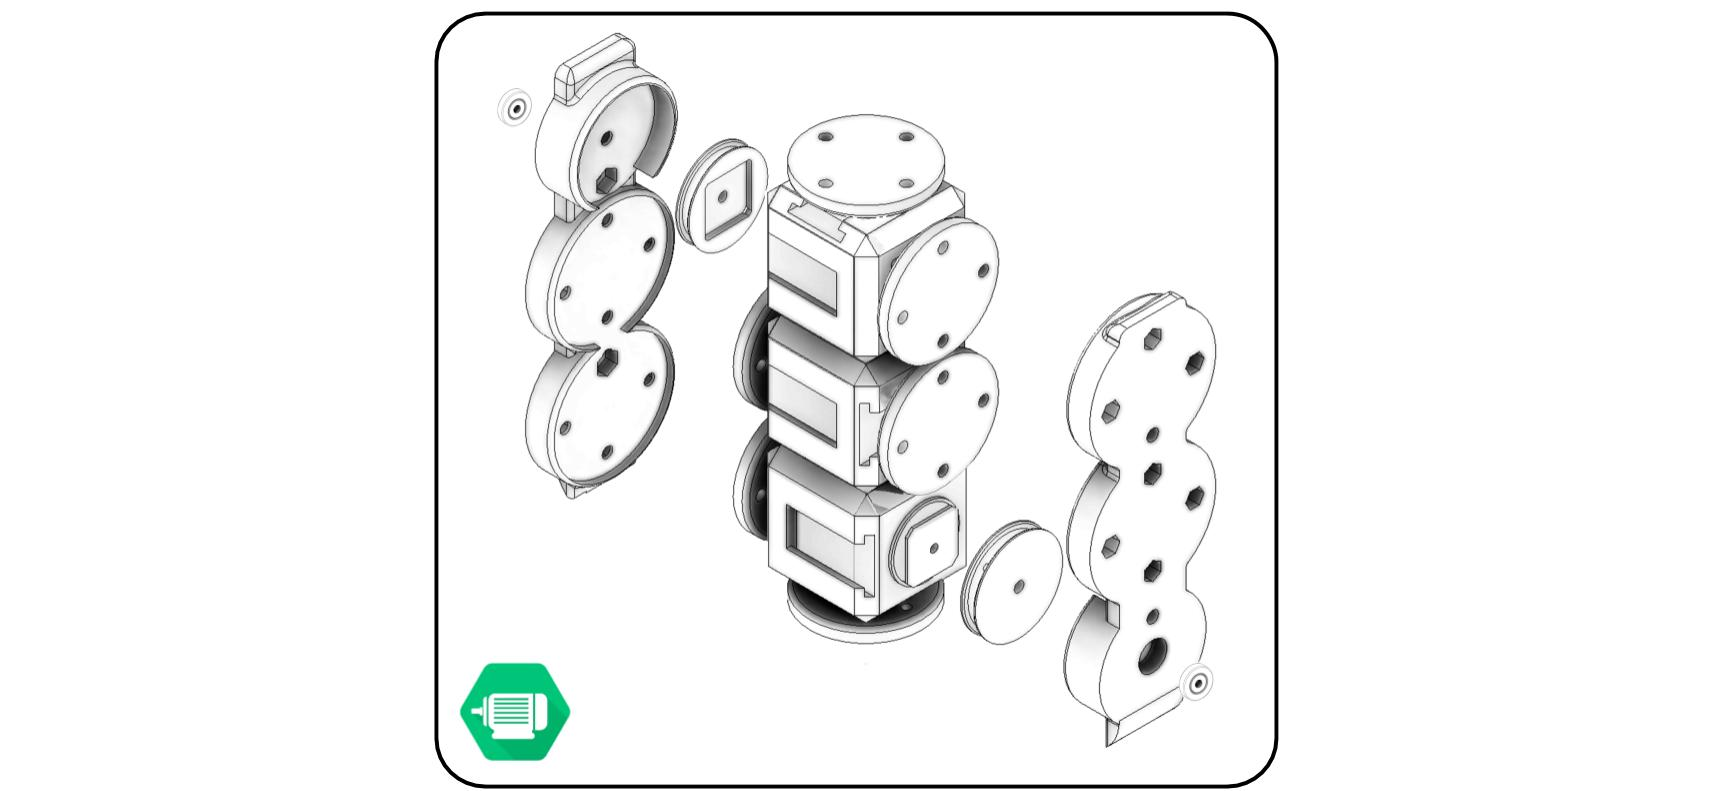
\includegraphics[width=\textwidth]{figuras/Imagenes_Electronica/anclaje_servos.jpg}
   		\caption{Representación de como se fijan los servos a la estructura}
   		\label{fig:Electronica:montaje_servos}
   		\immagesource{Autor}
   	\end{figure}

    Ambas placas, tanto la \ingles{shield} como la placa Arduino Mega van montadas sobre una plataforma aprovechando los anclajes de los servos, tal y como se presenta en la figura \ref{fig:Electronica:placas}.
    \\
   	\begin{figure}[H]
   		\centering
   		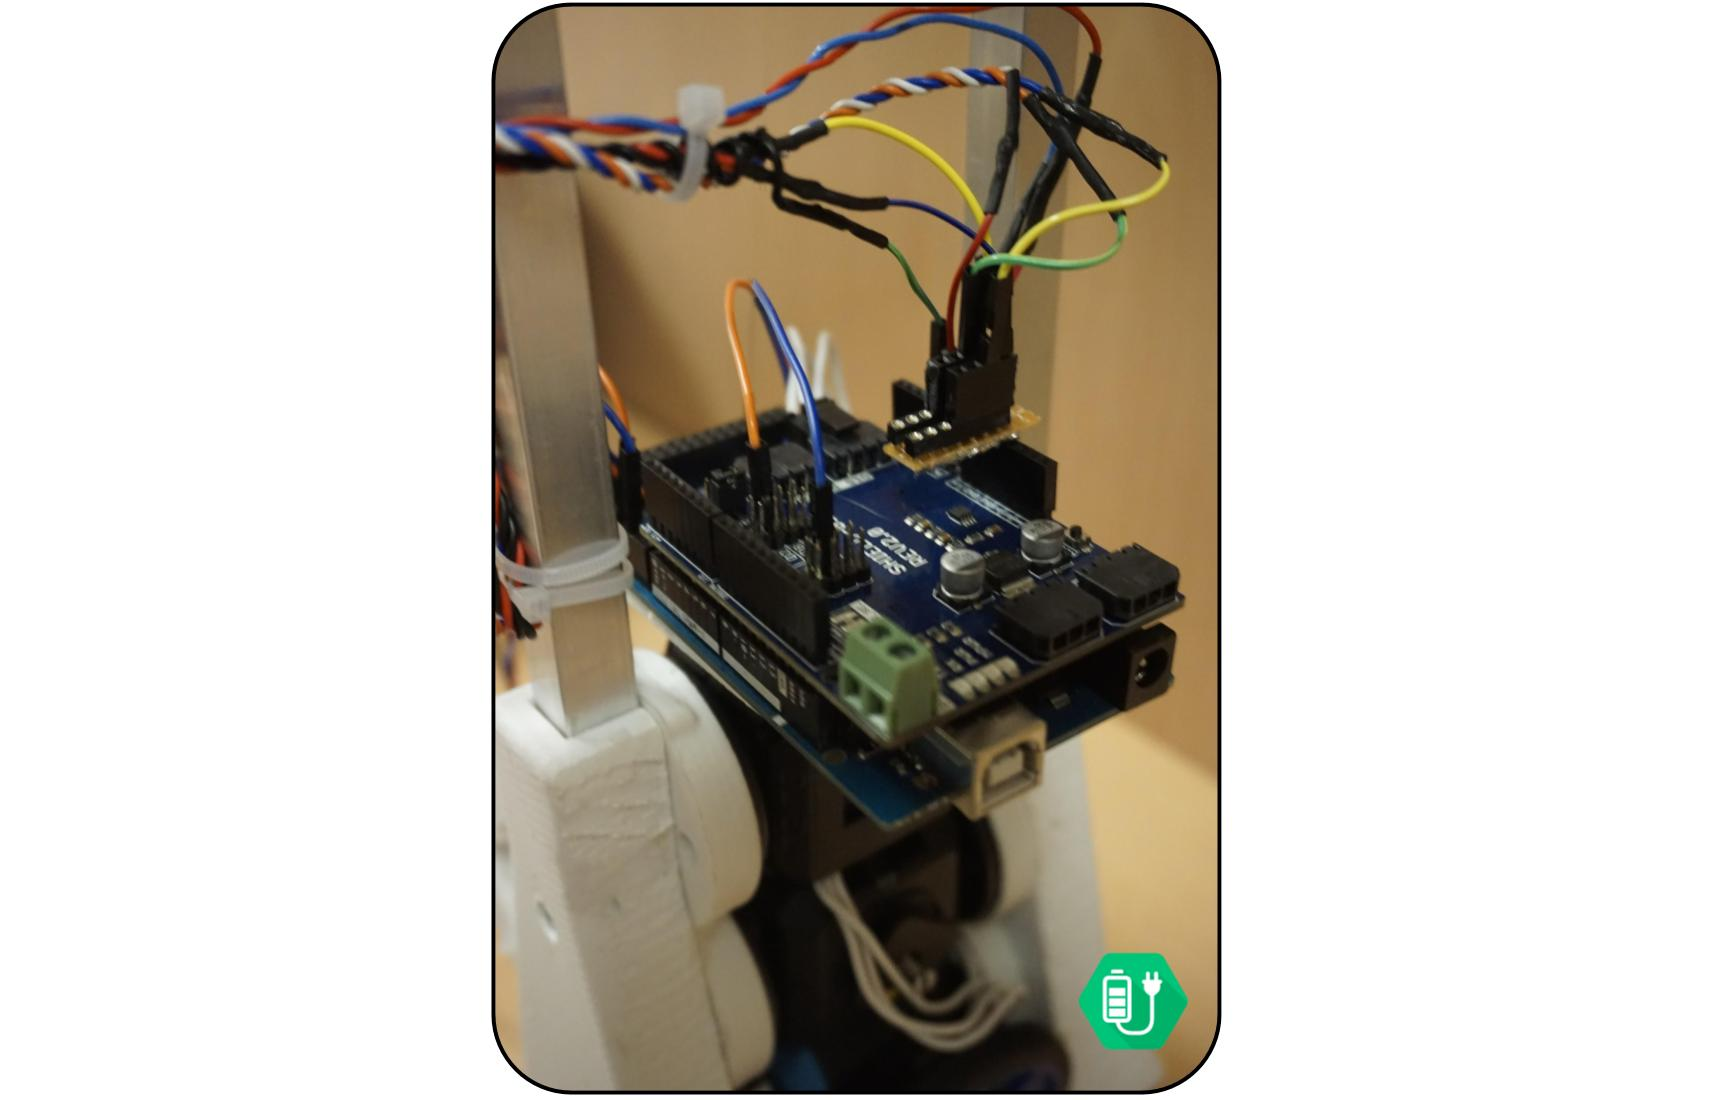
\includegraphics[width=\textwidth]{figuras/Imagenes_Electronica/foto_brazo_11.jpg}
   		\caption{Acoplamiento de las placas y motores}
   		\label{fig:Electronica:placas}
   		\immagesource{Autor}
   	\end{figure}
   	
    En el caso de los potenciómetros su montaje difiere de un caso a otro:
    \begin{itemize}
        \item Segunda Articulación: El movimiento de la articulación se transmite a través de un juego de engranajes hasta el potenciómetro, que está ubicado sobre el eje de dicha articulación. Se puede ver el montaje en la figura \ref{fig:Mecanica:realimentacion_1}. Se ha aprovechado el uso de engranajes para aumentar la resolución de medida de forma que el movimiento se amplifica para aprovechar en su totalidad los $265^o$ de giro ofrecidos por el potenciómetro. La relación entre las medidas se presenta a continuación:
        \begin{equation}
        	Medida Articular = \frac{Medida Potenciometro \cdot 180}{265}
        \end{equation}
        \item Tercera articulación: El eje del potenciómetro se encuentra en la misma línea que el eje de la articulación. Se ha diseñado una pieza para unir el eje del potenciómetro al giro de la barra que puede verse en la figura \ref{fig:Mecanica:realimentacion_2} En este caso la lectura leída del potenciómetro (en grados) es equivalente al desplazamiento articular.
    \end{itemize}

    \begin{minipage}{0.47\textwidth}
        \begin{figure}[H]
            \centering
            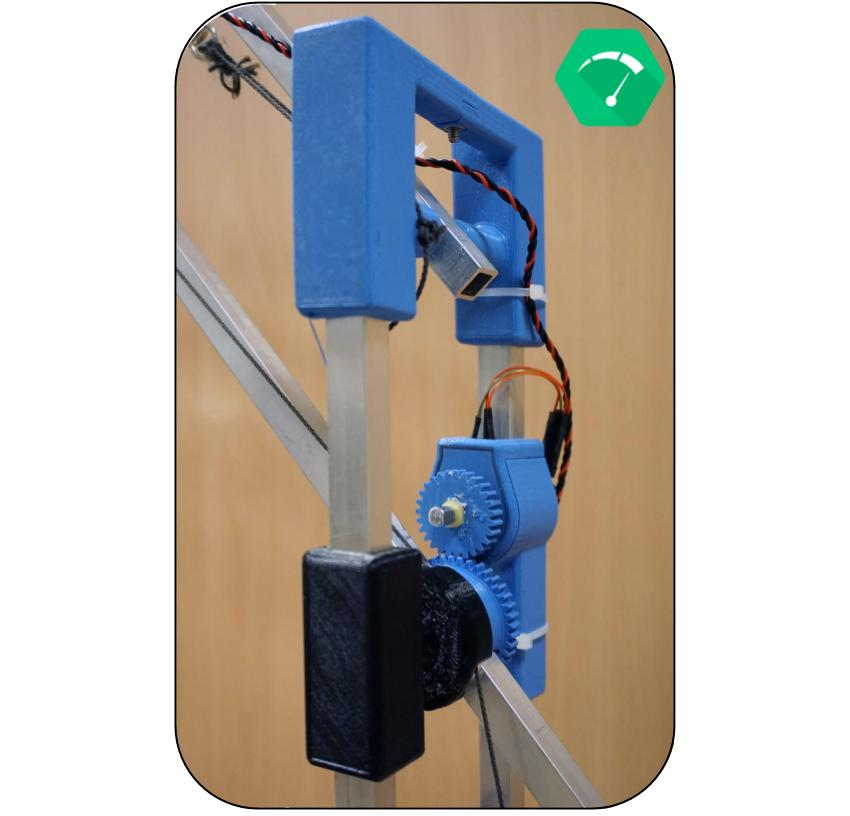
\includegraphics[width=1.15\textwidth]{figuras/Imagenes_Electronica/foto_brazo_3.jpg}
            \caption{Montaje de la realimentación para la segunda articulación}
            \label{fig:Mecanica:realimentacion_1}
            \immagesource{Autor}
        \end{figure}
    \end{minipage}
    \begin{minipage}{0.47\textwidth}\raggedright
        \begin{figure}[H]
            \centering
            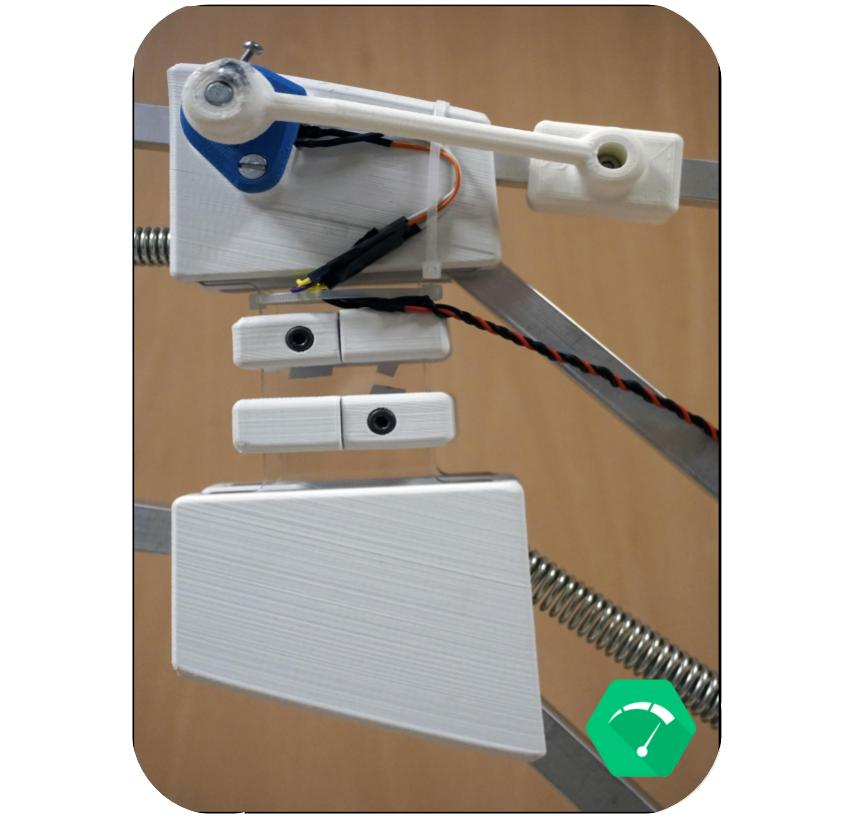
\includegraphics[width=1.15\textwidth]{figuras/Imagenes_Electronica/foto_brazo_2.jpg}
            \caption{Montaje de la realimentación para la tercera articulación}
            \label{fig:Mecanica:realimentacion_2}
            \immagesource{Autor}
        \end{figure}
    \end{minipage}
